% Copyright 2004 by Till Tantau <tantau@users.sourceforge.net>.
%
% In principle, this file can be redistributed and/or modified under
% the terms of the GNU Public License, version 2.
%
% However, this file is supposed to be a template to be modified
% for your own needs. For this reason, if you use this file as a
% template and not specifically distribute it as part of a another
% package/program, I grant the extra permission to freely copy and
% modify this file as you see fit and even to delete this copyright
% notice. 

\documentclass{beamer}

% There are many different themes available for Beamer. A comprehensive
% list with examples is given here:
% http://deic.uab.es/~iblanes/beamer_gallery/index_by_theme.html
% You can uncomment the themes below if you would like to use a different
% one:
\usetheme{Madrid}

% Customize Warsaw color 
\setbeamercolor*{palette primary}{use=structure,fg=white,bg=red!50!black}
\setbeamercolor*{palette secondary}{use=structure,fg=white,bg=red!60!black}
\setbeamercolor*{palette tertiary}{use=structure,fg=white,bg=red!70!black}

% Customize Warsaw block title and background colors
\setbeamercolor{block title}{bg=red!50!black,fg=white}

\title[Localization and Mapping]{Indoor Mobile Robot Localization and Mapping}

% % A subtitle is optional and this may be deleted
% \subtitle{Product Proposal}

\author[D.~Beebe]{Darrah~Beebe\\
Advisor: Dr. Suruz Miah}
% - Give the names in the same order as the appear in the paper.
% - Use the \inst{?} command only if the authors have different
%   affiliation.

\institute[Bradley University] % (optional, but mostly needed)
{
  Department of Electrical and Computer Engineering\\
  Bradley University\\
  1501 W. Bradley Avenue\\
  Peoria, IL, 61625, USA
}
% - Use the \inst command only if there are several affiliations.
% - Keep it simple, no one is interested in your street address.

\date[\today]{\today}
% - Either use conference name or its abbreviation.
% - Not really informative to the audience, more for people (including
%   yourself) who are reading the slides online

\logo{\hfill\href{http://www.bradley.edu}{
\includegraphics[width=0.75cm]{figs/logoBU1-Print}}}  % place logo in every page 


\subject{Mobile Robot Localization}
% This is only inserted into the PDF information catalog. Can be left
% out. 

% If you have a file called "university-logo-filename.xxx", where xxx
% is a graphic format that can be processed by latex or pdflatex,
% resp., then you can add a logo as follows:

% \pgfdeclareimage[height=0.5cm]{university-logo}{university-logo-filename}
% \logo{\pgfuseimage{university-logo}}

% Delete this, if you do not want the table of contents to pop up at
% the beginning of each subsection:
\AtBeginSubsection[]
{
  %\begin{frame}<beamer>{Outline}
  %  \tableofcontents[currentsection,currentsubsection]
  %\end{frame}
}

% Let's get started
\begin{document}

\begin{frame}
  \titlepage
\end{frame}

\begin{frame}{Outline}
  \tableofcontents
  % You might wish to add the option [pausesections]
\end{frame}

% Section and subsections will appear in the presentation overview
% and table of contents.
\section{Introduction}

\begin{frame}{Introduction}{}
  % applications of mobile robot navigation and problem description
  Goal of project is to implement XBee modules to to localize a mobile robot using Cayley-Menger determinant's based on signal strength.
\end{frame}

%----------------------------------

\section{Project So Far}

% put a slide with three dimensional system architecture drawing using ipe
% another slide with explanation

% put a slide with system block diagram

\subsection{Network Diagram}
\begin{frame}{Network Diagram}{Diagram of ZigBee network}

\begin{figure}
    \centering
    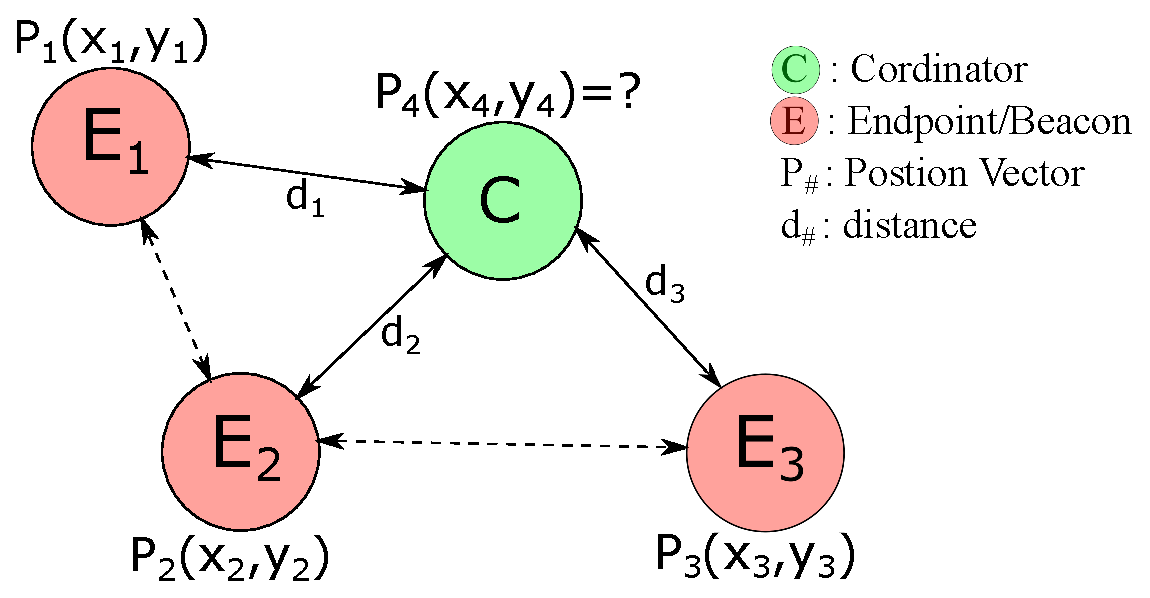
\includegraphics[scale=.6]{figs/inkscape/XBeeConectionDiagram_2}
    \caption{ZigBee network diagram}
    \label{fig:ZigBeeNetwork}
\end{figure}

\end{frame}

%----------------------------------

%\subsection{Diagram Breakdown}
%\begin{frame}{Diagram breakdown}
%    \begin{itemize}
%    \item
%    Configurable types\\
%    Coordinator (C), Router (R), Endpoint(E),
%    \item
%    Points P\textsubscript{1}, P\textsubscript{2}, and P\textsubscript{3} are known
%    P\textsubscript{4} is the unknown position of the mobile robot
%    \item
%    Distances d\textsubscript{1}, d\textsubscript{2}, and d\textsubscript{3} from dB reading
%    \end{itemize}
%\end{frame}

%----------------------------------

\subsection{Previously Done}
\begin{frame}{Previously Done}
    \begin{itemize}
    \item XCTU
    \item Powershell
    \item Backbone to XBee (linux c code)
    \item Calculate Distance - Ongoing
    \item Matrix Determinants Added - Ongoing
    \item File loading for beacon positions
    \item Trilateration equation implemented and Tested
    \end{itemize}
\end{frame}

\begin{frame}{Previously Done}
    \begin{figure}
    \centering
    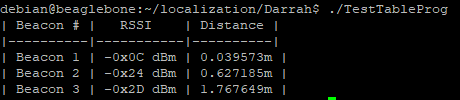
\includegraphics[scale=0.8]{figs/ScreenShots/RSSIOutputTableDist.PNG}
    \caption{RSSI+Distance(FreeSpace) Output Table}
    \label{fig:RSSIOutputTable_Darrah}
    \end{figure}
    
    \begin{figure}
    \centering
    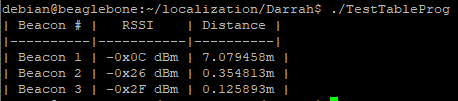
\includegraphics[scale=0.8]{figs/ScreenShots/RSSIOutputTableDist_2.PNG}
    \caption{RSSI+Distance(Miah Paper) Output Table}
    \label{fig:RSSIOutputTable_Paper}
    \end{figure}
    
    Note: Need to finish checking sources for "Miah Paper" solution
\end{frame}

%----------------------------------

\subsection{Current Progress}
\begin{frame}{Current Progress}
    \begin{itemize}
    \item Calculate Distance - Ongoing
    \item Fixed localization Program - Ongoing
    \end{itemize}
    
    \begin{figure}
    \centering
    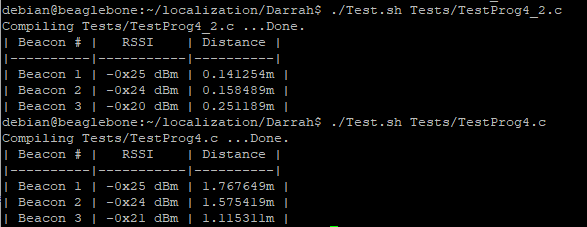
\includegraphics[scale=0.8]{figs/ScreenShots/DistanceFormulaOutputs.PNG}
    \caption{Current Distance Test Outputs}
    \label{fig:RSSIOutputTable_Paper}
    \end{figure}
\end{frame}

\subsection{Current Progress}
\begin{frame}{Current Progress}
    \begin{figure}
    \centering
    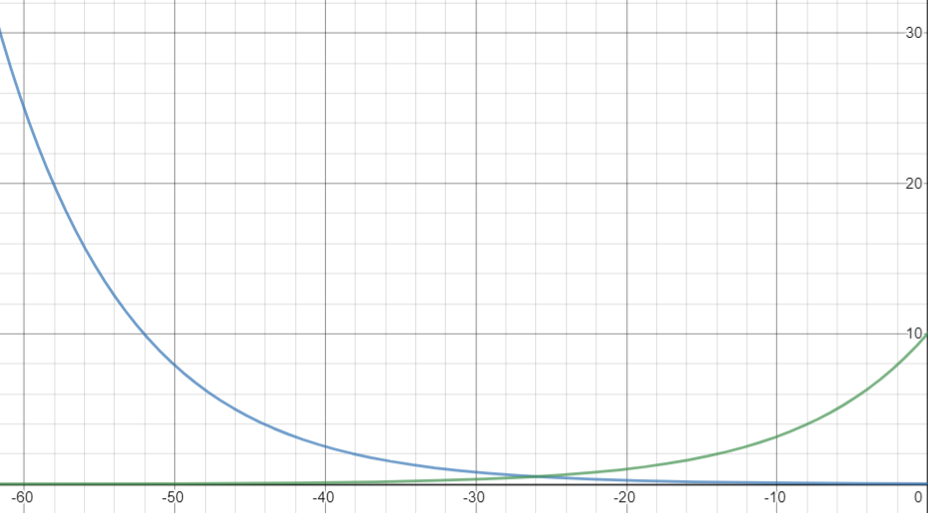
\includegraphics[scale=0.45]{figs/ScreenShots/GraphRepofRSSI.PNG}
    \caption{Current Distance Test Outputs}
    \label{fig:RSSIOutputTable_Paper}
    \end{figure}
\end{frame}

\begin{frame}{Current Progress}    
	\begin{figure}
    \centering
    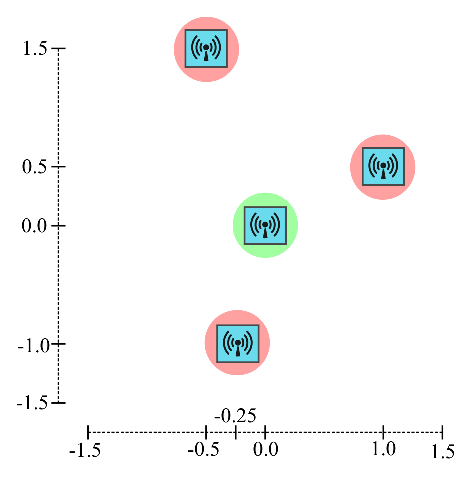
\includegraphics[scale=0.9]{figs/inkscape/TestSetup}
    \caption{Test Setup}
    \label{fig:Test Setup}
    \end{figure}
\end{frame}

\begin{frame}{Current Progress}    
	\begin{figure}
    \centering
    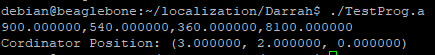
\includegraphics[scale=0.7]{figs/ScreenShots/LocalizationTestOutput.PNG}
    \caption{Old Distance Test Outputs}
    \label{fig:RSSIOutputTable_Paper}
	
    \centering
    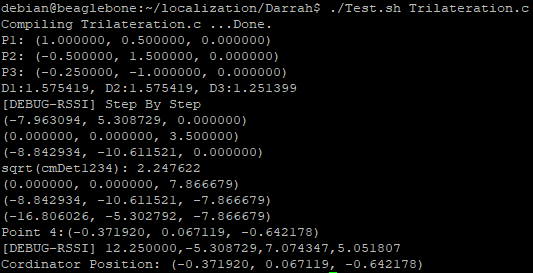
\includegraphics[scale=0.7]{figs/ScreenShots/PositionOutput.PNG}
    \caption{Current Distance Test Outputs}
    \label{fig:RSSIOutputTable_Paper}
    \end{figure}
\end{frame}

\subsection{Current Progress}
\begin{frame}{Current Progress}
	\begin{itemize}
    \item File Transfer Batch script
    \item Bit of extra cleanup/comments
    \end{itemize}
\end{frame}

%----------------------------------

\section{Future Directions}

\begin{frame}{Future Directions}{}
    \begin{itemize}
        \item Optimization/Consistency of localization program
        \item Putting together some API documentation
        \item Wiki Page
    \end{itemize}
\end{frame}

\end{document}


